\documentclass[]{article}

\usepackage{mathtools}
\usepackage{listings}
\usepackage{clrscode}
\usepackage{algorithm}
\usepackage{algorithmic}
\usepackage{graphicx}
\usepackage[top=2cm, bottom=2cm, left=2cm, right=2cm]{geometry}
\DeclareMathOperator*{\argmin}{arg\,min}
\DeclareMathOperator*{\argmax}{arg\,max}

\title{Homework 4}
\date{2015-12-1}
\author{Jingwei Zhang 201528013229095}

\begin{document}
    \maketitle
    \section{Problem 1}
    \begin{figure}[H]
        \centering
        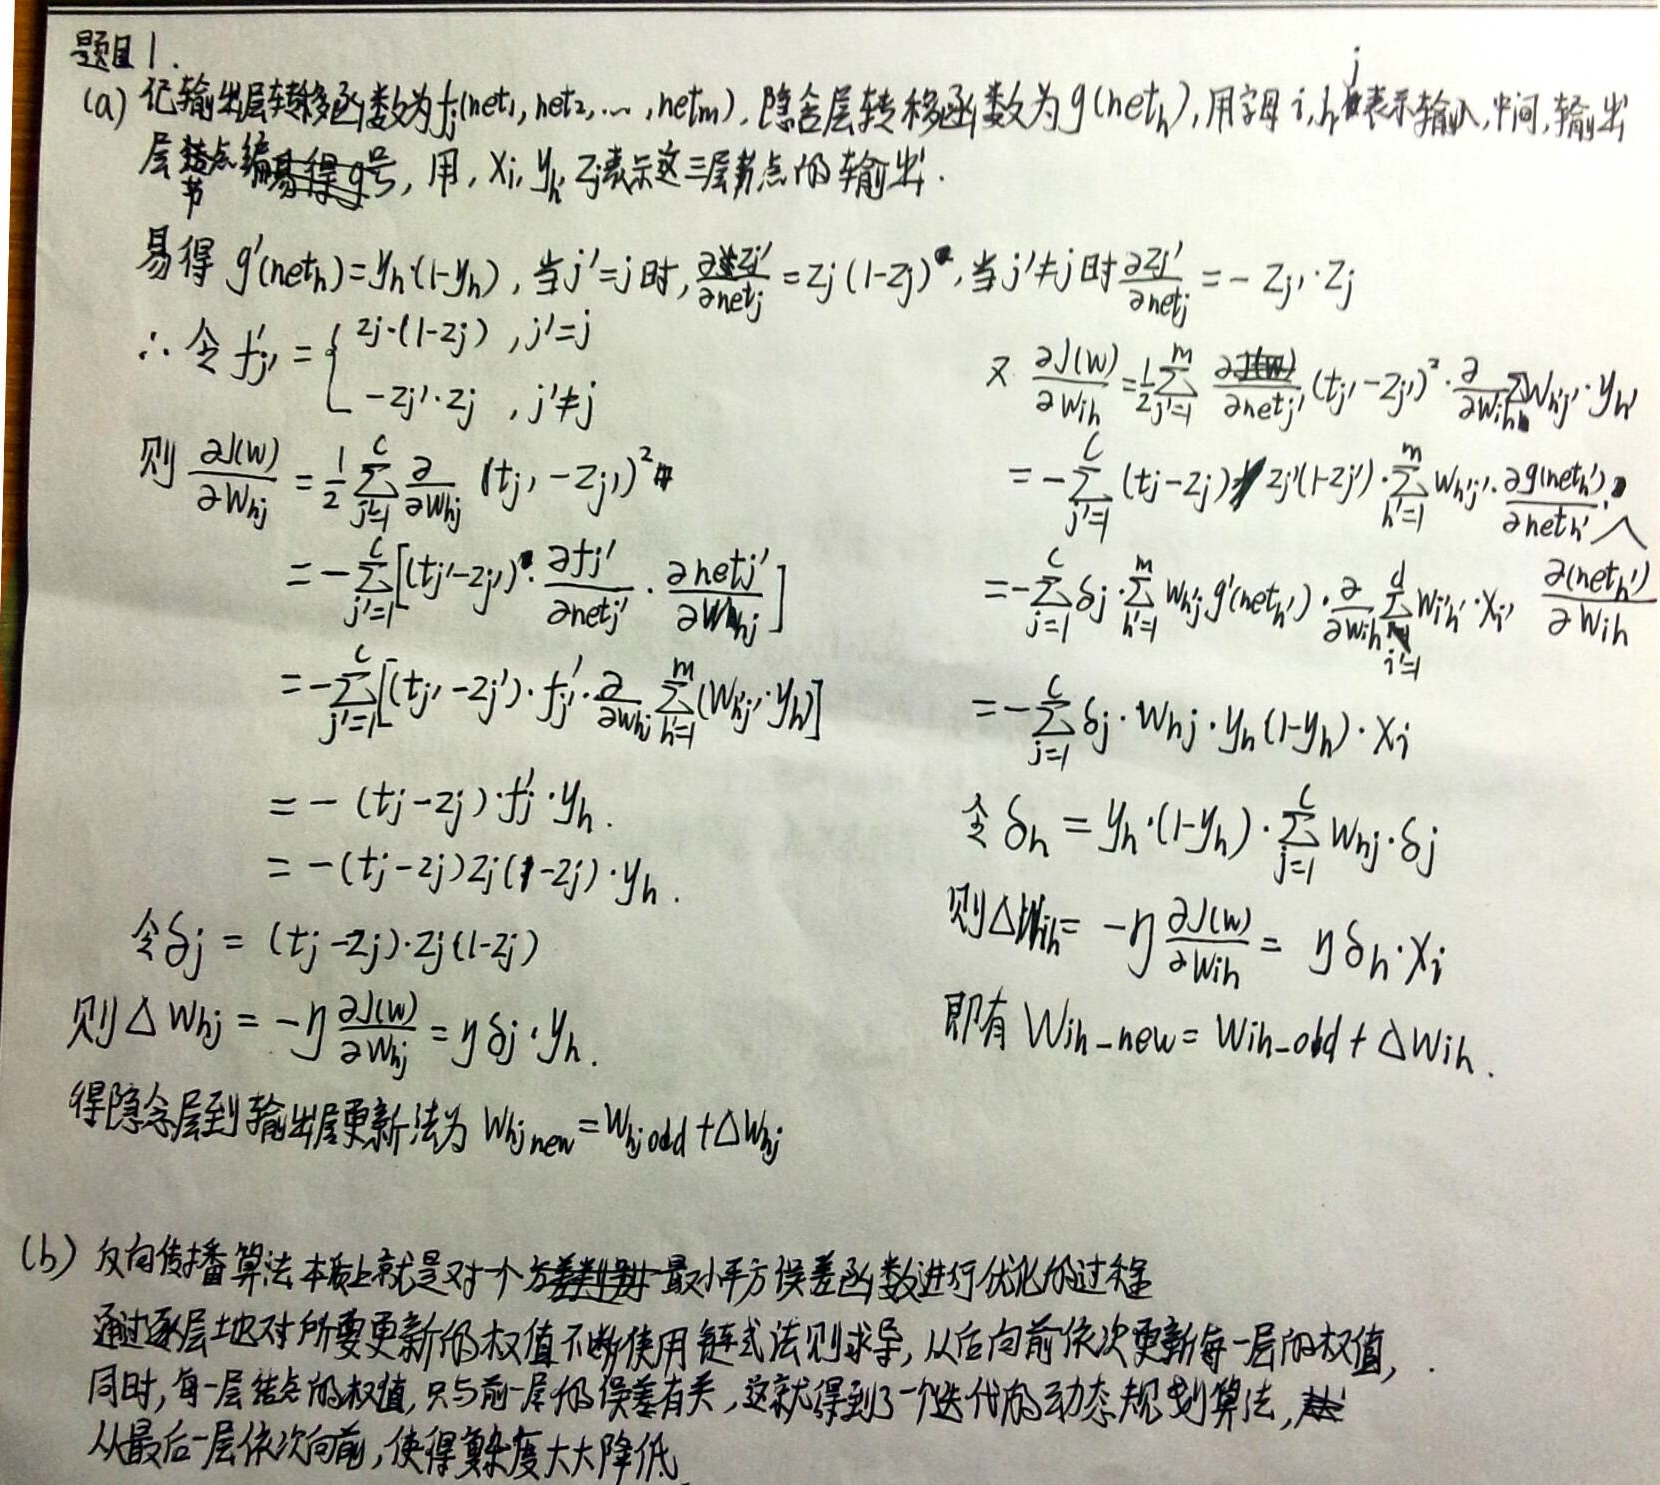
\includegraphics[scale=0.6]{P1.jpg}
    \end{figure}
    \section{Problem 2}
    \begin{figure}[H]
        \centering
        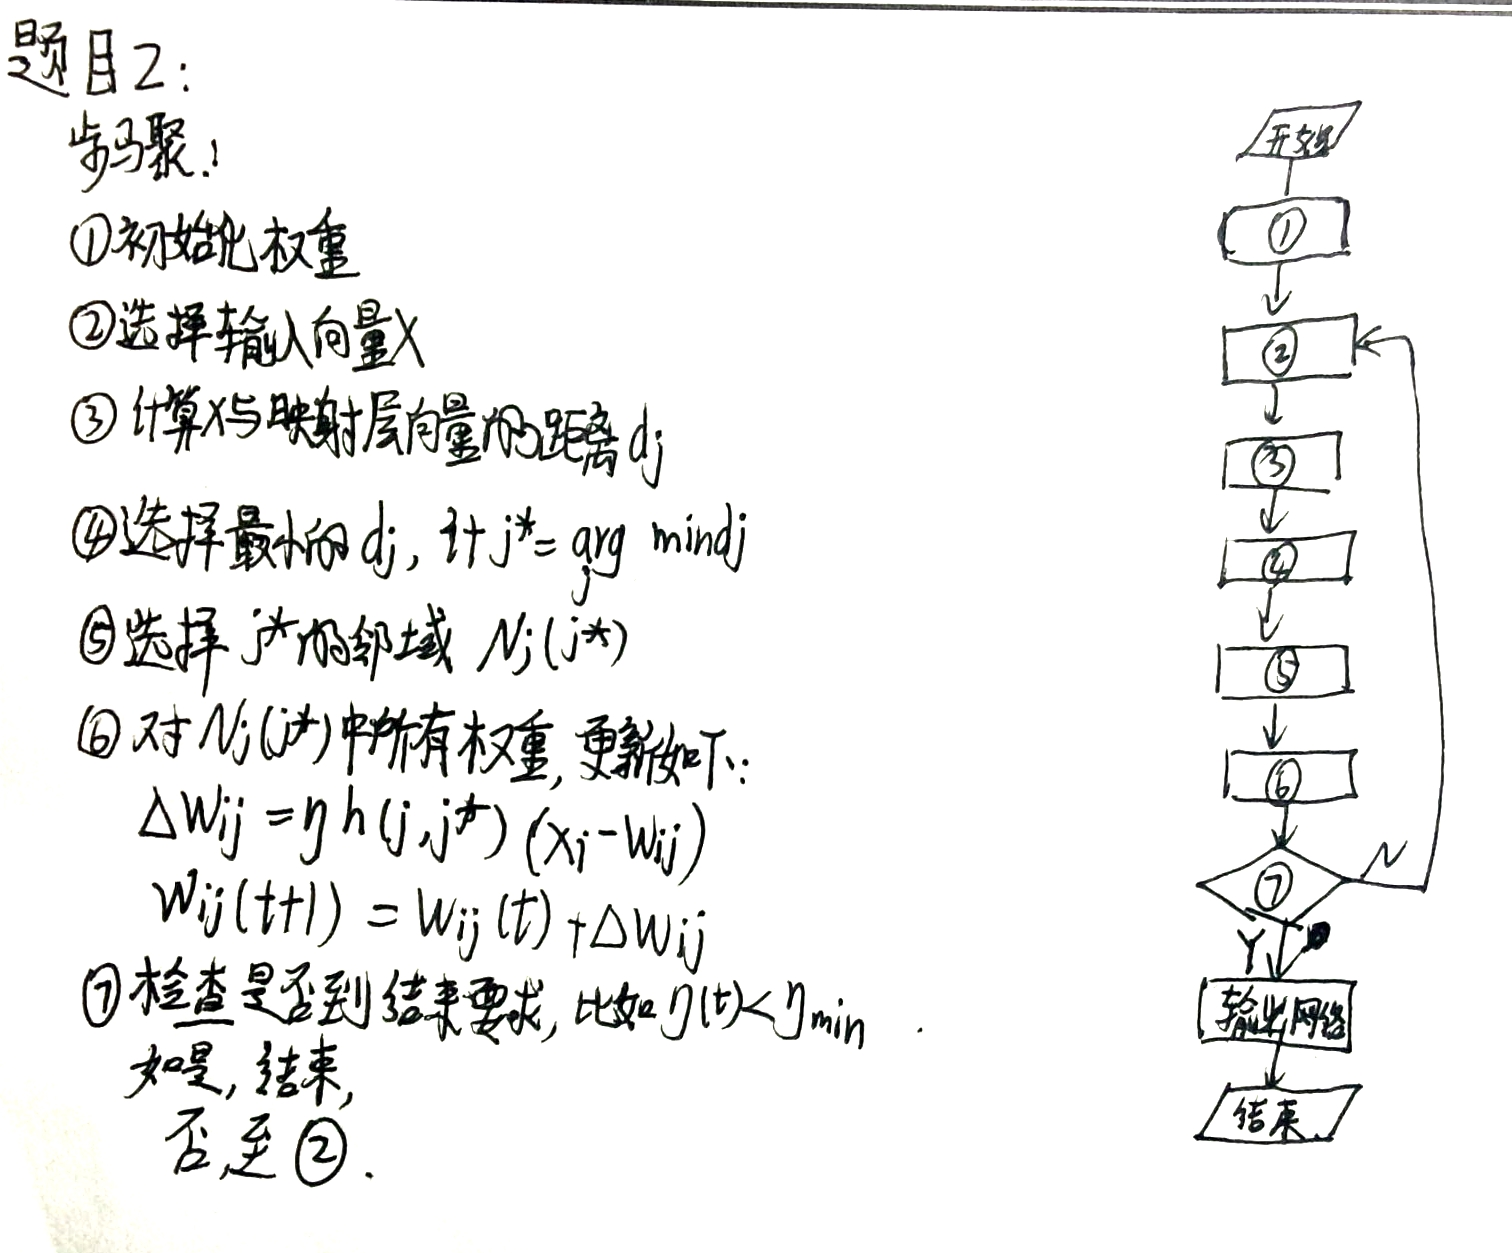
\includegraphics[scale=0.5]{P2.jpg}
    \end{figure}
    \section{Problem 3}
    \begin{figure}[H]
        \centering
        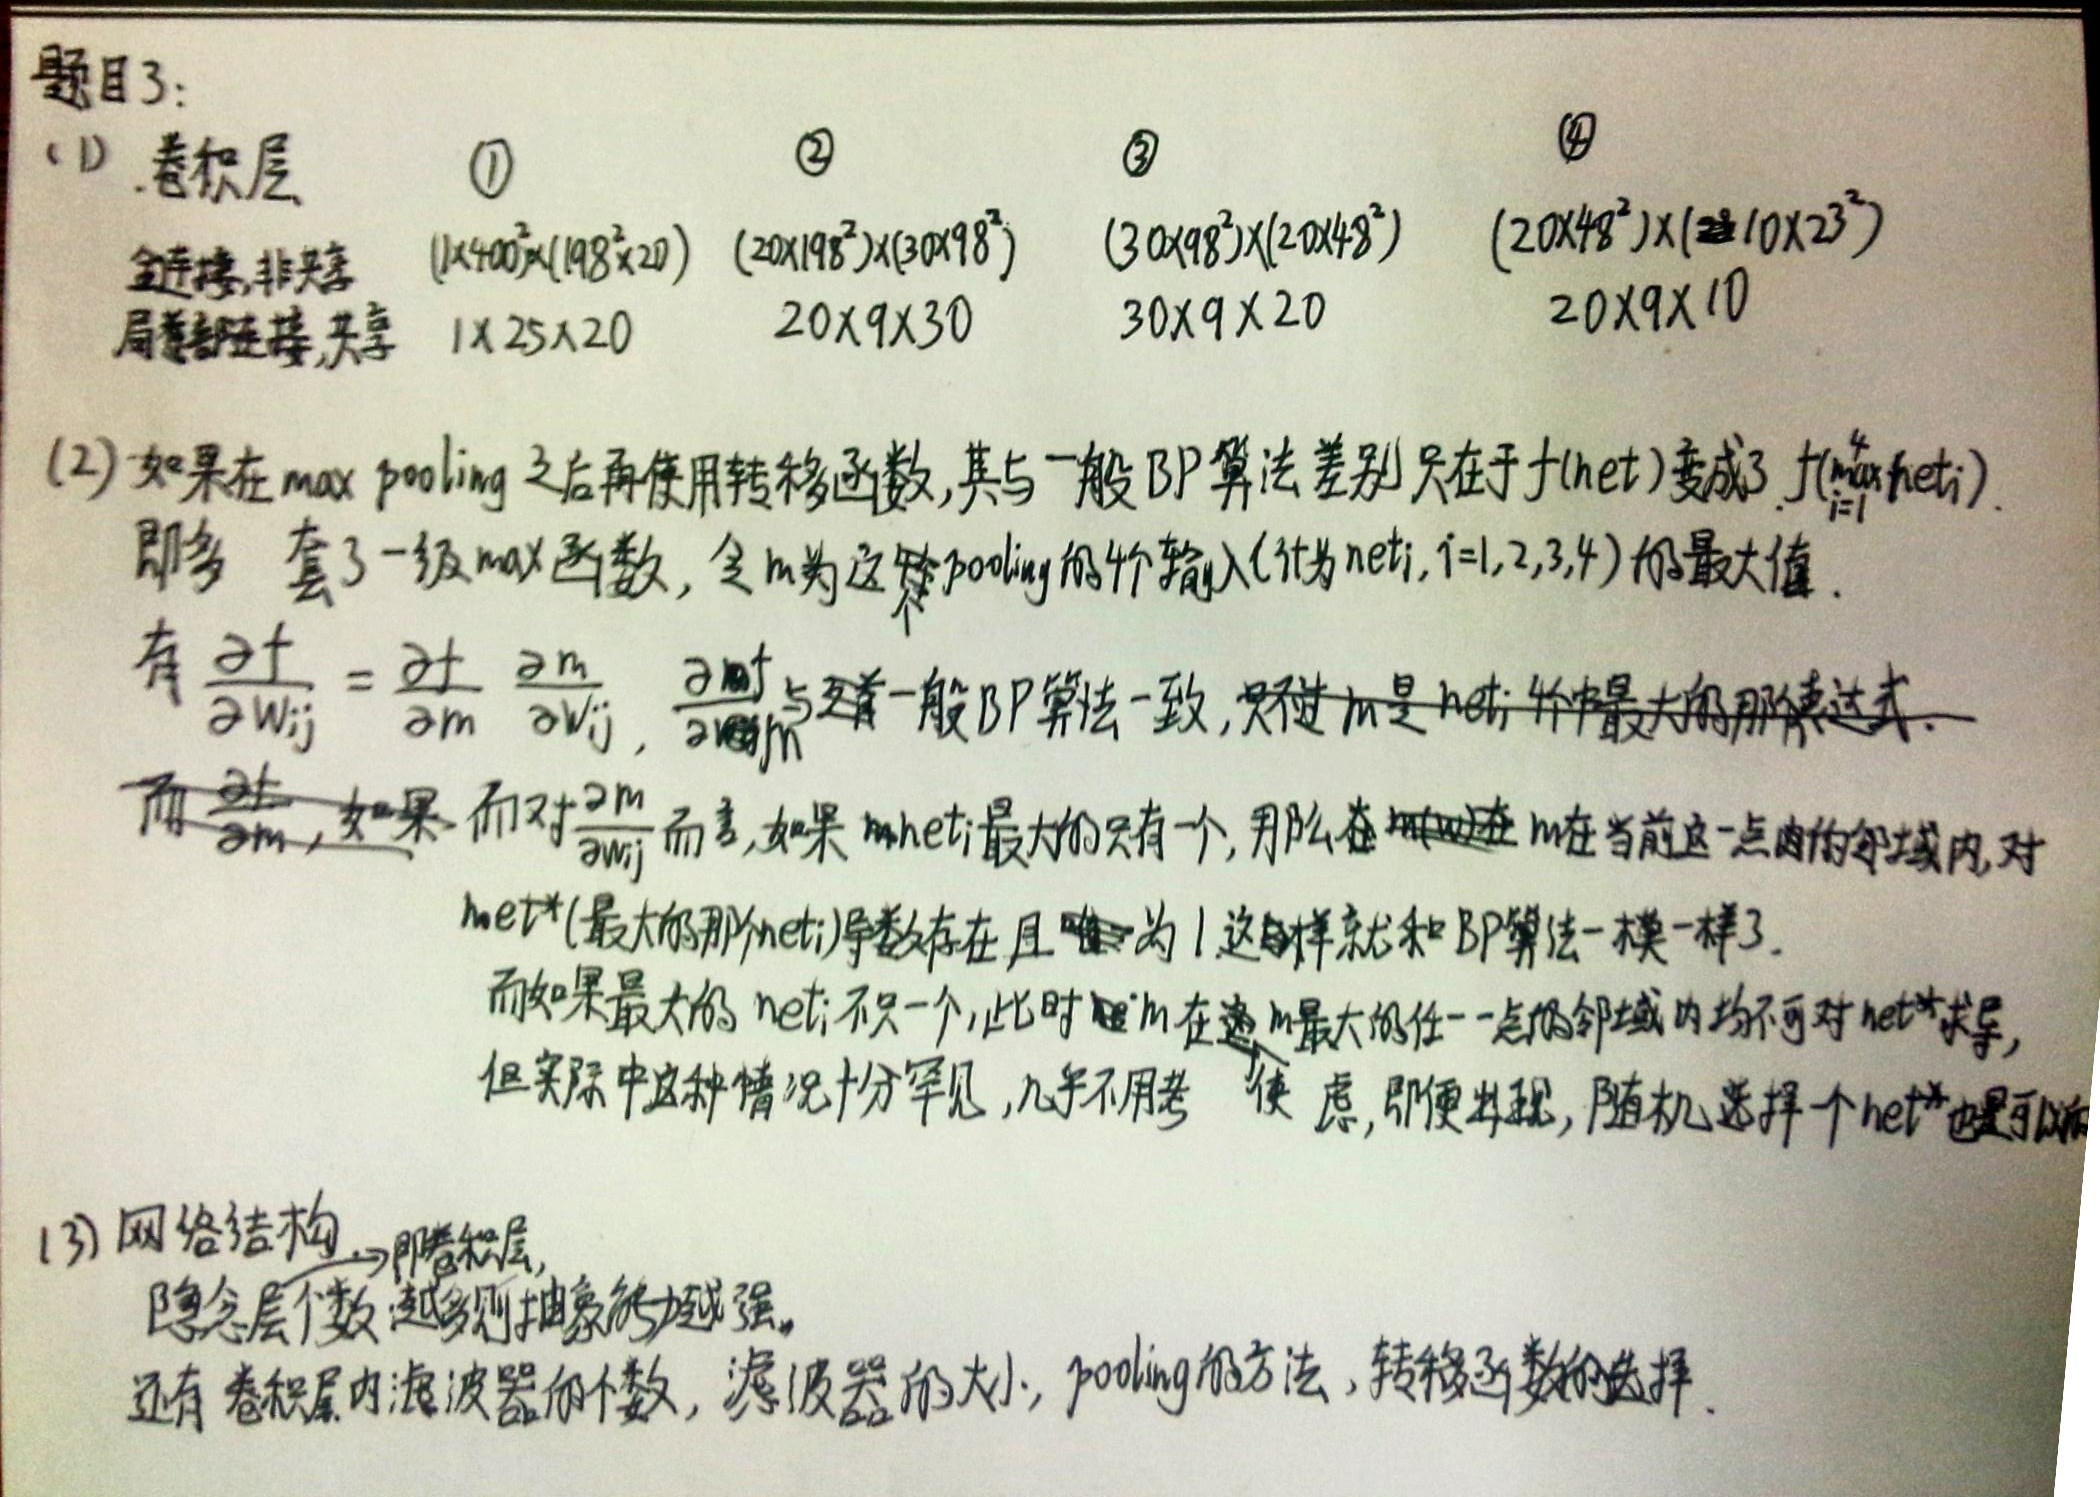
\includegraphics[scale=0.45]{P3.jpg}
    \end{figure}
    \section{Programming Problem 1}
    \subsection{Result}
    \paragraph{Question (a)}From my experiment, averagely, if the number of nodes in the hidden layer increases, the minimum of judge function will increase, though it requires more passes of training samples. It is difficult to draw a figure to show that trend, since all weights are initially random numbers.
    \paragraph{Question (b)}Effects of different $\eta$ have shown in Figures blow. From these two figures we can see that generally, when eta increases, the judging function will decrease to its minimum more quickly.
    \begin{figure}[H]
        \centering
        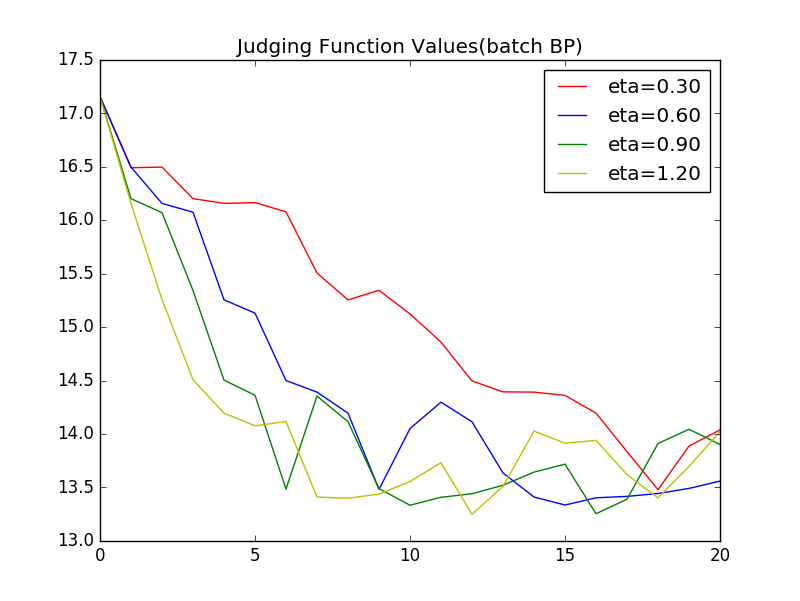
\includegraphics[scale=0.5]{PP1_batch.png}
        \caption{Figure for Batch BP}
    \end{figure}
    \begin{figure}[H]
        \centering
        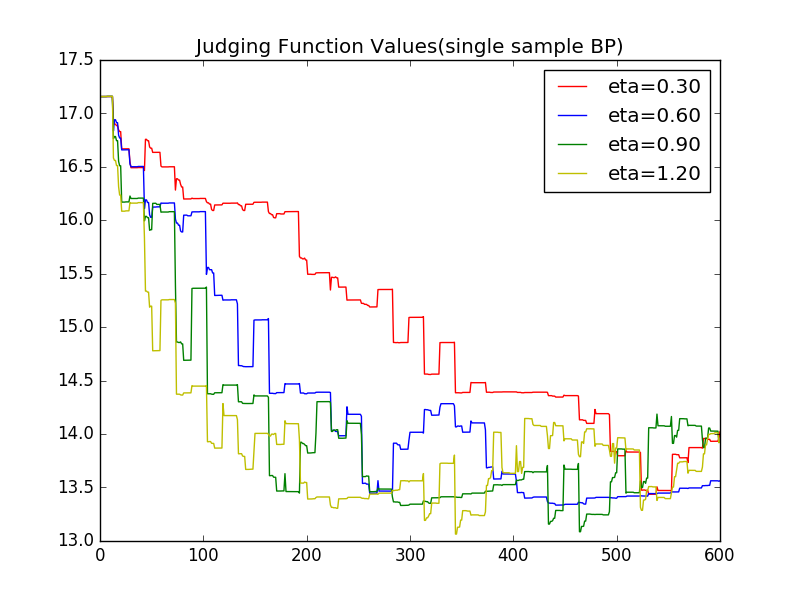
\includegraphics[scale=0.5]{PP1_single.png}
        \caption{Figure for Single Sample BP}
    \end{figure}  
    \paragraph{Question (c)}Figures are shown above.

    \subsection{Code}
    \lstinputlisting[language=Python]{1.py}


\end{document}